\documentclass[twoside]{book}

% Packages required by doxygen
\usepackage{fixltx2e}
\usepackage{calc}
\usepackage{doxygen}
\usepackage[export]{adjustbox} % also loads graphicx
\usepackage{graphicx}
\usepackage[utf8]{inputenc}
\usepackage{makeidx}
\usepackage{multicol}
\usepackage{multirow}
\PassOptionsToPackage{warn}{textcomp}
\usepackage{textcomp}
\usepackage[nointegrals]{wasysym}
\usepackage[table]{xcolor}

% Font selection
\usepackage[T1]{fontenc}
\usepackage[scaled=.90]{helvet}
\usepackage{courier}
\usepackage{amssymb}
\usepackage{sectsty}
\renewcommand{\familydefault}{\sfdefault}
\allsectionsfont{%
  \fontseries{bc}\selectfont%
  \color{darkgray}%
}
\renewcommand{\DoxyLabelFont}{%
  \fontseries{bc}\selectfont%
  \color{darkgray}%
}
\newcommand{\+}{\discretionary{\mbox{\scriptsize$\hookleftarrow$}}{}{}}

% Page & text layout
\usepackage{geometry}
\geometry{%
  a4paper,%
  top=2.5cm,%
  bottom=2.5cm,%
  left=2.5cm,%
  right=2.5cm%
}
\tolerance=750
\hfuzz=15pt
\hbadness=750
\setlength{\emergencystretch}{15pt}
\setlength{\parindent}{0cm}
\setlength{\parskip}{3ex plus 2ex minus 2ex}
\makeatletter
\renewcommand{\paragraph}{%
  \@startsection{paragraph}{4}{0ex}{-1.0ex}{1.0ex}{%
    \normalfont\normalsize\bfseries\SS@parafont%
  }%
}
\renewcommand{\subparagraph}{%
  \@startsection{subparagraph}{5}{0ex}{-1.0ex}{1.0ex}{%
    \normalfont\normalsize\bfseries\SS@subparafont%
  }%
}
\makeatother

% Headers & footers
\usepackage{fancyhdr}
\pagestyle{fancyplain}
\fancyhead[LE]{\fancyplain{}{\bfseries\thepage}}
\fancyhead[CE]{\fancyplain{}{}}
\fancyhead[RE]{\fancyplain{}{\bfseries\leftmark}}
\fancyhead[LO]{\fancyplain{}{\bfseries\rightmark}}
\fancyhead[CO]{\fancyplain{}{}}
\fancyhead[RO]{\fancyplain{}{\bfseries\thepage}}
\fancyfoot[LE]{\fancyplain{}{}}
\fancyfoot[CE]{\fancyplain{}{}}
\fancyfoot[RE]{\fancyplain{}{\bfseries\scriptsize Generated by Doxygen }}
\fancyfoot[LO]{\fancyplain{}{\bfseries\scriptsize Generated by Doxygen }}
\fancyfoot[CO]{\fancyplain{}{}}
\fancyfoot[RO]{\fancyplain{}{}}
\renewcommand{\footrulewidth}{0.4pt}
\renewcommand{\chaptermark}[1]{%
  \markboth{#1}{}%
}
\renewcommand{\sectionmark}[1]{%
  \markright{\thesection\ #1}%
}

% Indices & bibliography
\usepackage{natbib}
\usepackage[titles]{tocloft}
\setcounter{tocdepth}{3}
\setcounter{secnumdepth}{5}
\makeindex

% Hyperlinks (required, but should be loaded last)
\usepackage{ifpdf}
\ifpdf
  \usepackage[pdftex,pagebackref=true]{hyperref}
\else
  \usepackage[ps2pdf,pagebackref=true]{hyperref}
\fi
\hypersetup{%
  colorlinks=true,%
  linkcolor=blue,%
  citecolor=blue,%
  unicode%
}

% Custom commands
\newcommand{\clearemptydoublepage}{%
  \newpage{\pagestyle{empty}\cleardoublepage}%
}

\usepackage{caption}
\captionsetup{labelsep=space,justification=centering,font={bf},singlelinecheck=off,skip=4pt,position=top}

%===== C O N T E N T S =====

\begin{document}

% Titlepage & ToC
\hypersetup{pageanchor=false,
             bookmarksnumbered=true,
             pdfencoding=unicode
            }
\pagenumbering{roman}
\begin{titlepage}
\vspace*{7cm}
\begin{center}%
{\Large Turtlebot Navigator }\\
\vspace*{1cm}
{\large Generated by Doxygen 1.8.11}\\
\end{center}
\end{titlepage}
\clearemptydoublepage
\tableofcontents
\clearemptydoublepage
\pagenumbering{arabic}
\hypersetup{pageanchor=true}

%--- Begin generated contents ---
\chapter{L\+I\+C\+E\+N\+SE}
\label{md_src_turtlebot_navigator_LICENSE}
\hypertarget{md_src_turtlebot_navigator_LICENSE}{}
M\+IT License

Copyright (c) 2019 Arpit Aggarwal Shantam Bajpai

Permission is hereby granted, free of charge, to any person obtaining a copy of this software and associated documentation files (the \char`\"{}\+Software\char`\"{}), to deal in the Software without restriction, including without limitation the rights to use, copy, modify, merge, publish, distribute, sublicense, and/or sell copies of the Software, and to permit persons to whom the Software is furnished to do so, subject to the following conditions\+:

The above copyright notice and this permission notice shall be included in all copies or substantial portions of the Software.

T\+HE S\+O\+F\+T\+W\+A\+RE IS P\+R\+O\+V\+I\+D\+ED \char`\"{}\+A\+S I\+S\char`\"{}, W\+I\+T\+H\+O\+UT W\+A\+R\+R\+A\+N\+TY OF A\+NY K\+I\+ND, E\+X\+P\+R\+E\+SS OR I\+M\+P\+L\+I\+ED, I\+N\+C\+L\+U\+D\+I\+NG B\+UT N\+OT L\+I\+M\+I\+T\+ED TO T\+HE W\+A\+R\+R\+A\+N\+T\+I\+ES OF M\+E\+R\+C\+H\+A\+N\+T\+A\+B\+I\+L\+I\+TY, F\+I\+T\+N\+E\+SS F\+OR A P\+A\+R\+T\+I\+C\+U\+L\+AR P\+U\+R\+P\+O\+SE A\+ND N\+O\+N\+I\+N\+F\+R\+I\+N\+G\+E\+M\+E\+NT. IN NO E\+V\+E\+NT S\+H\+A\+LL T\+HE A\+U\+T\+H\+O\+RS OR C\+O\+P\+Y\+R\+I\+G\+HT H\+O\+L\+D\+E\+RS BE L\+I\+A\+B\+LE F\+OR A\+NY C\+L\+A\+IM, D\+A\+M\+A\+G\+ES OR O\+T\+H\+ER L\+I\+A\+B\+I\+L\+I\+TY, W\+H\+E\+T\+H\+ER IN AN A\+C\+T\+I\+ON OF C\+O\+N\+T\+R\+A\+CT, T\+O\+RT OR O\+T\+H\+E\+R\+W\+I\+SE, A\+R\+I\+S\+I\+NG F\+R\+OM, O\+UT OF OR IN C\+O\+N\+N\+E\+C\+T\+I\+ON W\+I\+TH T\+HE S\+O\+F\+T\+W\+A\+RE OR T\+HE U\+SE OR O\+T\+H\+ER D\+E\+A\+L\+I\+N\+GS IN T\+HE S\+O\+F\+T\+W\+A\+RE. 
\chapter{Turtlebot Navigator}
\label{md_src_turtlebot_navigator_readme}
\hypertarget{md_src_turtlebot_navigator_readme}{}
\href{https://travis-ci.org/arp95/enpm808x_turtlebot_navigator}{\tt } \href{https://coveralls.io/github/arp95/enpm808x_turtlebot_navigator?branch=master}{\tt } \subsection*{\hyperlink{_l_i_c_e_n_s_e_8md}{L\+I\+C\+E\+N\+S\+E.\+md} \char`\"{}!\mbox{[}\+Packagist\mbox{]}(https\+://img.\+shields.\+io/packagist/l/doctrine/orm.\+svg)\char`\"{} }

\subsection*{About the Authors}

Shantam Bajpai\+: I am a first year graduate student pursuing my masters degree in Robotics from the University of Maryland, College Park. Prior to joining University of Maryland I completed my undergraduate in Electrical and Electronics Engineering from Vellore Institute of Technology, Vellore, India.

Arpit Aggarwal\+: I am a first year graduate student pursuing my masters degree in Robotics from the University of Maryland, College Park. Prior to joining University of Maryland I completed my undergraduate in Electrical Engineering from Delhi Technological University, Delhi, India.

\subsection*{Overview of the project}

Turtlebots are small robots that can drive around and sense their environment through a microsoft kinect sensor mounted on its body. This is an inspection robot for Acme Robotics which acts as an automated surveillance system providing security in a variety of environments. The robot navigates an unknown indoor environment and creates a real time 3-\/D map of the environment in the form of a point cloud using S\+L\+A\+M(\+Simultaneous Localization and Mapping). The robot uses the turtlebot package and the octomap package to develop the 3D map.

\subsection*{Dependencies}

The following dependencies are required to run this package\+:


\begin{DoxyEnumerate}
\item R\+OS kinetic
\item catkin (\href{http://wiki.ros.org/catkin#Installing_catkin}{\tt http\+://wiki.\+ros.\+org/catkin\#\+Installing\+\_\+catkin})
\item Ubuntu 16.\+04 For installing R\+OS (\href{http://wiki.ros.org/kinetic/Installation}{\tt http\+://wiki.\+ros.\+org/kinetic/\+Installation})
\end{DoxyEnumerate}

\#\# Standard install via command-\/line 
\begin{DoxyCode}
1 cd ~/catkin\_ws/src
2 git clone --recursive https://github.com/arp95/enpm808x\_turtlebot\_navigator
3 cd ..
4 catkin\_make
\end{DoxyCode}


\subsection*{Agile Iterative Process}

\href{https://docs.google.com/spreadsheets/d/1Gf2HPhlzFCxhdOP1XlNDx23QuuKKL7okn-5ru6TXR6c/edit?usp=sharing}{\tt } 
\chapter{Class Index}
\section{Class List}
Here are the classes, structs, unions and interfaces with brief descriptions\+:\begin{DoxyCompactList}
\item\contentsline{section}{\hyperlink{class_navigation}{Navigation} }{\pageref{class_navigation}}{}
\item\contentsline{section}{\hyperlink{class_obstacle_detector}{Obstacle\+Detector} }{\pageref{class_obstacle_detector}}{}
\end{DoxyCompactList}

\chapter{File Index}
\section{File List}
Here is a list of all files with brief descriptions\+:\begin{DoxyCompactList}
\item\contentsline{section}{src/turtlebot\+\_\+navigator/include/\hyperlink{_navigation_8h}{Navigation.\+h} \\*Describes the \hyperlink{class_navigation}{Navigation} class }{\pageref{_navigation_8h}}{}
\item\contentsline{section}{src/turtlebot\+\_\+navigator/include/\hyperlink{_obstacle_detector_8h}{Obstacle\+Detector.\+h} \\*Defines the \hyperlink{class_obstacle_detector}{Obstacle\+Detector} class }{\pageref{_obstacle_detector_8h}}{}
\item\contentsline{section}{src/turtlebot\+\_\+navigator/src/\hyperlink{src_2main_8cpp}{main.\+cpp} }{\pageref{src_2main_8cpp}}{}
\item\contentsline{section}{src/turtlebot\+\_\+navigator/src/\hyperlink{_navigation_8cpp}{Navigation.\+cpp} \\*Describes the \hyperlink{class_navigation}{Navigation} class }{\pageref{_navigation_8cpp}}{}
\item\contentsline{section}{src/turtlebot\+\_\+navigator/src/\hyperlink{_obstacle_detector_8cpp}{Obstacle\+Detector.\+cpp} \\*Implements the methods of the \hyperlink{class_obstacle_detector}{Obstacle\+Detector} class }{\pageref{_obstacle_detector_8cpp}}{}
\item\contentsline{section}{src/turtlebot\+\_\+navigator/test/\hyperlink{test_2main_8cpp}{main.\+cpp} }{\pageref{test_2main_8cpp}}{}
\item\contentsline{section}{src/turtlebot\+\_\+navigator/test/\hyperlink{_navigation_test_8cpp}{Navigation\+Test.\+cpp} \\*Test cases for \hyperlink{_navigation_test_8cpp}{Navigation\+Test.\+cpp} file }{\pageref{_navigation_test_8cpp}}{}
\item\contentsline{section}{src/turtlebot\+\_\+navigator/test/\hyperlink{_obstacle_detector_test_8cpp}{Obstacle\+Detector\+Test.\+cpp} \\*Test cases for \hyperlink{_obstacle_detector_8cpp}{Obstacle\+Detector.\+cpp} file }{\pageref{_obstacle_detector_test_8cpp}}{}
\end{DoxyCompactList}

\chapter{Class Documentation}
\hypertarget{class_navigation}{}\section{Navigation Class Reference}
\label{class_navigation}\index{Navigation@{Navigation}}


{\ttfamily \#include $<$Navigation.\+h$>$}

\subsection*{Public Member Functions}
\begin{DoxyCompactItemize}
\item 
\hyperlink{class_navigation_a81fdffdefe46340da5fa6c570066b42b}{Navigation} ()
\item 
void \hyperlink{class_navigation_a1a0954420883674ce5e676d700ebc572}{move} (bool detect)
\item 
\hyperlink{class_navigation_addd4022d716df48f4e55a1db69361ba7}{$\sim$\+Navigation} ()
\end{DoxyCompactItemize}


\subsection{Constructor \& Destructor Documentation}
\index{Navigation@{Navigation}!Navigation@{Navigation}}
\index{Navigation@{Navigation}!Navigation@{Navigation}}
\subsubsection[{\texorpdfstring{Navigation()}{Navigation()}}]{\setlength{\rightskip}{0pt plus 5cm}Navigation\+::\+Navigation (
\begin{DoxyParamCaption}
{}
\end{DoxyParamCaption}
)}\hypertarget{class_navigation_a81fdffdefe46340da5fa6c570066b42b}{}\label{class_navigation_a81fdffdefe46340da5fa6c570066b42b}
\index{Navigation@{Navigation}!````~Navigation@{$\sim$\+Navigation}}
\index{````~Navigation@{$\sim$\+Navigation}!Navigation@{Navigation}}
\subsubsection[{\texorpdfstring{$\sim$\+Navigation()}{~Navigation()}}]{\setlength{\rightskip}{0pt plus 5cm}Navigation\+::$\sim$\+Navigation (
\begin{DoxyParamCaption}
{}
\end{DoxyParamCaption}
)}\hypertarget{class_navigation_addd4022d716df48f4e55a1db69361ba7}{}\label{class_navigation_addd4022d716df48f4e55a1db69361ba7}


\subsection{Member Function Documentation}
\index{Navigation@{Navigation}!move@{move}}
\index{move@{move}!Navigation@{Navigation}}
\subsubsection[{\texorpdfstring{move(bool detect)}{move(bool detect)}}]{\setlength{\rightskip}{0pt plus 5cm}void Navigation\+::move (
\begin{DoxyParamCaption}
\item[{bool}]{detect}
\end{DoxyParamCaption}
)}\hypertarget{class_navigation_a1a0954420883674ce5e676d700ebc572}{}\label{class_navigation_a1a0954420883674ce5e676d700ebc572}


The documentation for this class was generated from the following files\+:\begin{DoxyCompactItemize}
\item 
src/turtlebot\+\_\+navigator/include/\hyperlink{_navigation_8h}{Navigation.\+h}\item 
src/turtlebot\+\_\+navigator/src/\hyperlink{_navigation_8cpp}{Navigation.\+cpp}\end{DoxyCompactItemize}

\hypertarget{class_obstacle_detector}{}\section{Obstacle\+Detector Class Reference}
\label{class_obstacle_detector}\index{Obstacle\+Detector@{Obstacle\+Detector}}


{\ttfamily \#include $<$Obstacle\+Detector.\+h$>$}

\subsection*{Public Member Functions}
\begin{DoxyCompactItemize}
\item 
\hyperlink{class_obstacle_detector_ae97e1085c7f6a3418faa1295c81d0b87}{Obstacle\+Detector} ()
\begin{DoxyCompactList}\small\item\em Constructs the \hyperlink{class_obstacle_detector}{Obstacle\+Detector} object. \end{DoxyCompactList}\item 
\hyperlink{class_obstacle_detector_aa3b42649fc5c973f677a4aba968d25cc}{$\sim$\+Obstacle\+Detector} ()
\begin{DoxyCompactList}\small\item\em Destructor of the \hyperlink{class_obstacle_detector}{Obstacle\+Detector} class. \end{DoxyCompactList}\item 
void \hyperlink{class_obstacle_detector_adac40fe27cffd6e331d1e97e7b6ca24b}{laser\+Callback} (const sensor\+\_\+msgs\+::\+Laser\+Scan\+::\+Const\+Ptr \&data)
\begin{DoxyCompactList}\small\item\em Callback for ros subscriber sub. \end{DoxyCompactList}\item 
void \hyperlink{class_obstacle_detector_af30f1b30086872b68b446e54052534b2}{dist\+Callback} (const std\+\_\+msgs\+::\+Float64\+::\+Const\+Ptr \&data)
\begin{DoxyCompactList}\small\item\em Callback for ros subscriber dist\+Sub. \end{DoxyCompactList}\item 
bool \hyperlink{class_obstacle_detector_aede4ced75212e4c1f57ded5ebb0db52d}{get\+Is\+Collision} ()
\begin{DoxyCompactList}\small\item\em Returns the value of is\+Collision. \end{DoxyCompactList}\item 
void \hyperlink{class_obstacle_detector_affe63dc23f2365c719f788689798598d}{set\+Is\+Collision} (bool collision\+Val)
\begin{DoxyCompactList}\small\item\em Returns the value of is\+Collision. \end{DoxyCompactList}\end{DoxyCompactItemize}


\subsection{Constructor \& Destructor Documentation}
\index{Obstacle\+Detector@{Obstacle\+Detector}!Obstacle\+Detector@{Obstacle\+Detector}}
\index{Obstacle\+Detector@{Obstacle\+Detector}!Obstacle\+Detector@{Obstacle\+Detector}}
\subsubsection[{\texorpdfstring{Obstacle\+Detector()}{ObstacleDetector()}}]{\setlength{\rightskip}{0pt plus 5cm}Obstacle\+Detector\+::\+Obstacle\+Detector (
\begin{DoxyParamCaption}
{}
\end{DoxyParamCaption}
)\hspace{0.3cm}{\ttfamily [explicit]}}\hypertarget{class_obstacle_detector_ae97e1085c7f6a3418faa1295c81d0b87}{}\label{class_obstacle_detector_ae97e1085c7f6a3418faa1295c81d0b87}


Constructs the \hyperlink{class_obstacle_detector}{Obstacle\+Detector} object. 

\index{Obstacle\+Detector@{Obstacle\+Detector}!````~Obstacle\+Detector@{$\sim$\+Obstacle\+Detector}}
\index{````~Obstacle\+Detector@{$\sim$\+Obstacle\+Detector}!Obstacle\+Detector@{Obstacle\+Detector}}
\subsubsection[{\texorpdfstring{$\sim$\+Obstacle\+Detector()}{~ObstacleDetector()}}]{\setlength{\rightskip}{0pt plus 5cm}Obstacle\+Detector\+::$\sim$\+Obstacle\+Detector (
\begin{DoxyParamCaption}
{}
\end{DoxyParamCaption}
)}\hypertarget{class_obstacle_detector_aa3b42649fc5c973f677a4aba968d25cc}{}\label{class_obstacle_detector_aa3b42649fc5c973f677a4aba968d25cc}


Destructor of the \hyperlink{class_obstacle_detector}{Obstacle\+Detector} class. 



\subsection{Member Function Documentation}
\index{Obstacle\+Detector@{Obstacle\+Detector}!dist\+Callback@{dist\+Callback}}
\index{dist\+Callback@{dist\+Callback}!Obstacle\+Detector@{Obstacle\+Detector}}
\subsubsection[{\texorpdfstring{dist\+Callback(const std\+\_\+msgs\+::\+Float64\+::\+Const\+Ptr \&data)}{distCallback(const std_msgs::Float64::ConstPtr &data)}}]{\setlength{\rightskip}{0pt plus 5cm}void Obstacle\+Detector\+::dist\+Callback (
\begin{DoxyParamCaption}
\item[{const std\+\_\+msgs\+::\+Float64\+::\+Const\+Ptr \&}]{data}
\end{DoxyParamCaption}
)}\hypertarget{class_obstacle_detector_af30f1b30086872b68b446e54052534b2}{}\label{class_obstacle_detector_af30f1b30086872b68b446e54052534b2}


Callback for ros subscriber dist\+Sub. 


\begin{DoxyParams}{Parameters}
{\em data} & const std\+\_\+msgs\+::\+Float64\+::\+Const\+Ptr. \\
\hline
\end{DoxyParams}
\index{Obstacle\+Detector@{Obstacle\+Detector}!get\+Is\+Collision@{get\+Is\+Collision}}
\index{get\+Is\+Collision@{get\+Is\+Collision}!Obstacle\+Detector@{Obstacle\+Detector}}
\subsubsection[{\texorpdfstring{get\+Is\+Collision()}{getIsCollision()}}]{\setlength{\rightskip}{0pt plus 5cm}bool Obstacle\+Detector\+::get\+Is\+Collision (
\begin{DoxyParamCaption}
{}
\end{DoxyParamCaption}
)}\hypertarget{class_obstacle_detector_aede4ced75212e4c1f57ded5ebb0db52d}{}\label{class_obstacle_detector_aede4ced75212e4c1f57ded5ebb0db52d}


Returns the value of is\+Collision. 

\index{Obstacle\+Detector@{Obstacle\+Detector}!laser\+Callback@{laser\+Callback}}
\index{laser\+Callback@{laser\+Callback}!Obstacle\+Detector@{Obstacle\+Detector}}
\subsubsection[{\texorpdfstring{laser\+Callback(const sensor\+\_\+msgs\+::\+Laser\+Scan\+::\+Const\+Ptr \&data)}{laserCallback(const sensor_msgs::LaserScan::ConstPtr &data)}}]{\setlength{\rightskip}{0pt plus 5cm}void Obstacle\+Detector\+::laser\+Callback (
\begin{DoxyParamCaption}
\item[{const sensor\+\_\+msgs\+::\+Laser\+Scan\+::\+Const\+Ptr \&}]{data}
\end{DoxyParamCaption}
)}\hypertarget{class_obstacle_detector_adac40fe27cffd6e331d1e97e7b6ca24b}{}\label{class_obstacle_detector_adac40fe27cffd6e331d1e97e7b6ca24b}


Callback for ros subscriber sub. 


\begin{DoxyParams}{Parameters}
{\em data} & sensor\+\_\+msgs\+::\+Laser\+Scan\+::\+Const\+Ptr. \\
\hline
\end{DoxyParams}
\index{Obstacle\+Detector@{Obstacle\+Detector}!set\+Is\+Collision@{set\+Is\+Collision}}
\index{set\+Is\+Collision@{set\+Is\+Collision}!Obstacle\+Detector@{Obstacle\+Detector}}
\subsubsection[{\texorpdfstring{set\+Is\+Collision(bool collision\+Val)}{setIsCollision(bool collisionVal)}}]{\setlength{\rightskip}{0pt plus 5cm}void Obstacle\+Detector\+::set\+Is\+Collision (
\begin{DoxyParamCaption}
\item[{bool}]{collision\+Val}
\end{DoxyParamCaption}
)}\hypertarget{class_obstacle_detector_affe63dc23f2365c719f788689798598d}{}\label{class_obstacle_detector_affe63dc23f2365c719f788689798598d}


Returns the value of is\+Collision. 


\begin{DoxyParams}{Parameters}
{\em collision\+Val} & bool. \\
\hline
\end{DoxyParams}


The documentation for this class was generated from the following files\+:\begin{DoxyCompactItemize}
\item 
src/turtlebot\+\_\+navigator/include/\hyperlink{_obstacle_detector_8h}{Obstacle\+Detector.\+h}\item 
src/turtlebot\+\_\+navigator/src/\hyperlink{_obstacle_detector_8cpp}{Obstacle\+Detector.\+cpp}\end{DoxyCompactItemize}

\chapter{File Documentation}
\hypertarget{_navigation_8h}{}\section{src/turtlebot\+\_\+navigator/include/\+Navigation.h File Reference}
\label{_navigation_8h}\index{src/turtlebot\+\_\+navigator/include/\+Navigation.\+h@{src/turtlebot\+\_\+navigator/include/\+Navigation.\+h}}


Describes the \hyperlink{class_navigation}{Navigation} class.  


{\ttfamily \#include $<$iostream$>$}\\*
{\ttfamily \#include $<$ros/ros.\+h$>$}\\*
{\ttfamily \#include $<$geometry\+\_\+msgs/\+Twist.\+h$>$}\\*
{\ttfamily \#include $<$Obstacle\+Detector.\+h$>$}\\*
Include dependency graph for Navigation.\+h\+:
\nopagebreak
\begin{figure}[H]
\begin{center}
\leavevmode
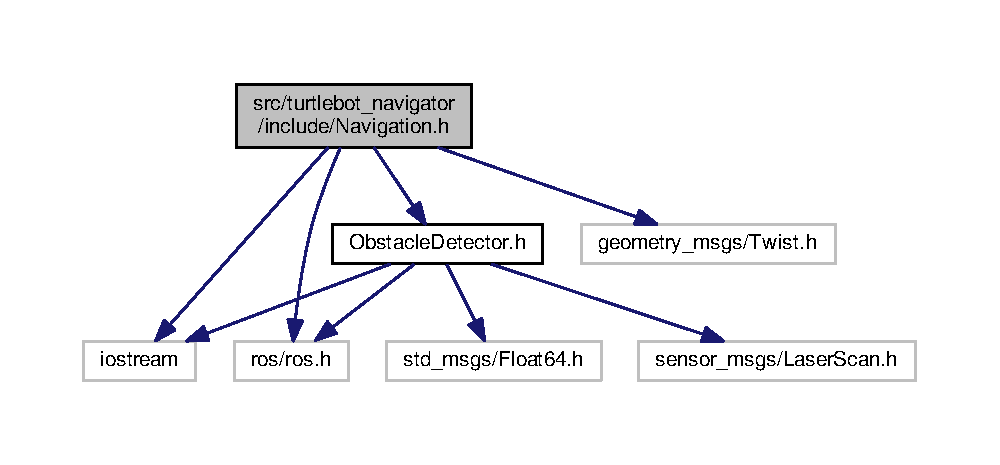
\includegraphics[width=350pt]{_navigation_8h__incl}
\end{center}
\end{figure}
This graph shows which files directly or indirectly include this file\+:
\nopagebreak
\begin{figure}[H]
\begin{center}
\leavevmode
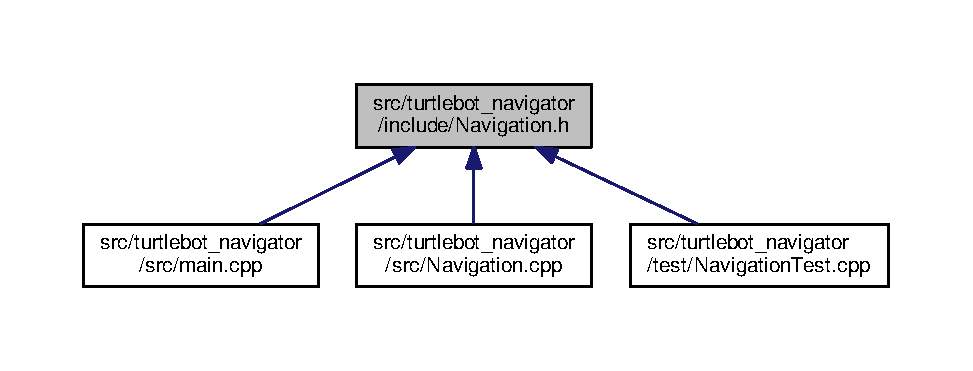
\includegraphics[width=350pt]{_navigation_8h__dep__incl}
\end{center}
\end{figure}
\subsection*{Classes}
\begin{DoxyCompactItemize}
\item 
class \hyperlink{class_navigation}{Navigation}
\end{DoxyCompactItemize}


\subsection{Detailed Description}
Describes the \hyperlink{class_navigation}{Navigation} class. 

M\+IT License

Copyright (c) 2019 Arpit Aggarwal Shantam Bajpai

Permission is hereby granted, free of charge, to any person obtaining a copy of this software and associated documentation files (the \char`\"{}\+Software\char`\"{}), to deal in the Software without restriction, including without limitation the rights to use, copy, modify, merge, publish, distribute, sublicense, and/or sell copies of the Software, and to permit persons to whom the Software is furnished to do so, subject to the following conditions\+:

The above copyright notice and this permission notice shall be included in all copies or substantial portions of the Software.

T\+HE S\+O\+F\+T\+W\+A\+RE IS P\+R\+O\+V\+I\+D\+ED \char`\"{}\+A\+S I\+S\char`\"{}, W\+I\+T\+H\+O\+UT W\+A\+R\+R\+A\+N\+TY OF A\+NY K\+I\+ND, E\+X\+P\+R\+E\+SS OR I\+M\+P\+L\+I\+ED, I\+N\+C\+L\+U\+D\+I\+NG B\+UT N\+OT L\+I\+M\+I\+T\+ED TO T\+HE W\+A\+R\+R\+A\+N\+T\+I\+ES OF M\+E\+R\+C\+H\+A\+N\+T\+A\+B\+I\+L\+I\+TY, F\+I\+T\+N\+E\+SS F\+OR A P\+A\+R\+T\+I\+C\+U\+L\+AR P\+U\+R\+P\+O\+SE A\+ND N\+O\+N\+I\+N\+F\+R\+I\+N\+G\+E\+M\+E\+NT. IN NO E\+V\+E\+NT S\+H\+A\+LL T\+HE A\+U\+T\+H\+O\+RS OR C\+O\+P\+Y\+R\+I\+G\+HT H\+O\+L\+D\+E\+RS BE L\+I\+A\+B\+LE F\+OR A\+NY C\+L\+A\+IM, D\+A\+M\+A\+G\+ES OR O\+T\+H\+ER L\+I\+A\+B\+I\+L\+I\+TY, W\+H\+E\+T\+H\+ER IN AN A\+C\+T\+I\+ON OF C\+O\+N\+T\+R\+A\+CT, T\+O\+RT OR O\+T\+H\+E\+R\+W\+I\+SE, A\+R\+I\+S\+I\+NG F\+R\+OM, O\+UT OF OR IN C\+O\+N\+N\+E\+C\+T\+I\+ON W\+I\+TH T\+HE S\+O\+F\+T\+W\+A\+RE OR T\+HE U\+SE OR O\+T\+H\+ER D\+E\+A\+L\+I\+N\+GS IN T\+HE S\+O\+F\+T\+W\+A\+RE.

\begin{DoxyCopyright}{Copyright}
M\+IT License 
\end{DoxyCopyright}

\hypertarget{_obstacle_detector_8h}{}\section{src/turtlebot\+\_\+navigator/include/\+Obstacle\+Detector.h File Reference}
\label{_obstacle_detector_8h}\index{src/turtlebot\+\_\+navigator/include/\+Obstacle\+Detector.\+h@{src/turtlebot\+\_\+navigator/include/\+Obstacle\+Detector.\+h}}


Defines the \hyperlink{class_obstacle_detector}{Obstacle\+Detector} class.  


{\ttfamily \#include $<$iostream$>$}\\*
{\ttfamily \#include $<$ros/ros.\+h$>$}\\*
{\ttfamily \#include $<$std\+\_\+msgs/\+Float64.\+h$>$}\\*
{\ttfamily \#include $<$sensor\+\_\+msgs/\+Laser\+Scan.\+h$>$}\\*
Include dependency graph for Obstacle\+Detector.\+h\+:
\nopagebreak
\begin{figure}[H]
\begin{center}
\leavevmode
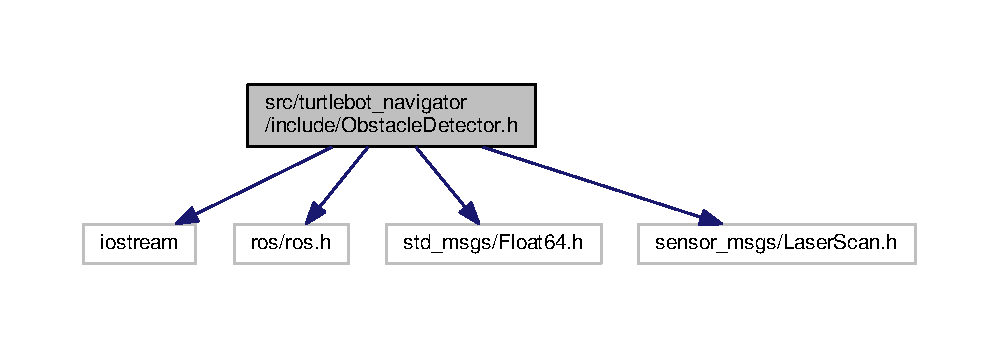
\includegraphics[width=350pt]{_obstacle_detector_8h__incl}
\end{center}
\end{figure}
This graph shows which files directly or indirectly include this file\+:
\nopagebreak
\begin{figure}[H]
\begin{center}
\leavevmode
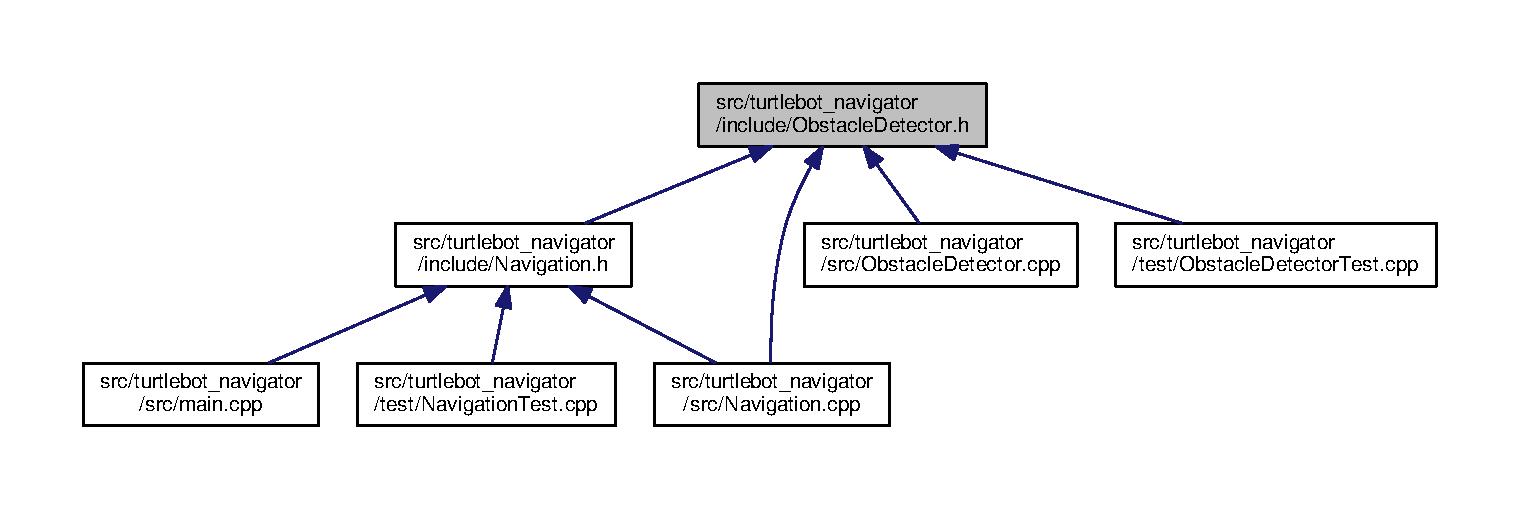
\includegraphics[width=350pt]{_obstacle_detector_8h__dep__incl}
\end{center}
\end{figure}
\subsection*{Classes}
\begin{DoxyCompactItemize}
\item 
class \hyperlink{class_obstacle_detector}{Obstacle\+Detector}
\end{DoxyCompactItemize}


\subsection{Detailed Description}
Defines the \hyperlink{class_obstacle_detector}{Obstacle\+Detector} class. 

M\+IT License

Copyright (c) 2019 Arpit Aggarwal Shantam Bajpai

Permission is hereby granted, free of charge, to any person obtaining a copy of this software and associated documentation files (the \char`\"{}\+Software\char`\"{}), to deal in the Software without restriction, including without limitation the rights to use, copy, modify, merge, publish, distribute, sublicense, and/or sell copies of the Software, and to permit persons to whom the Software is furnished to do so, subject to the following conditions\+:

The above copyright notice and this permission notice shall be included in all copies or substantial portions of the Software.

T\+HE S\+O\+F\+T\+W\+A\+RE IS P\+R\+O\+V\+I\+D\+ED \char`\"{}\+A\+S I\+S\char`\"{}, W\+I\+T\+H\+O\+UT W\+A\+R\+R\+A\+N\+TY OF A\+NY K\+I\+ND, E\+X\+P\+R\+E\+SS OR I\+M\+P\+L\+I\+ED, I\+N\+C\+L\+U\+D\+I\+NG B\+UT N\+OT L\+I\+M\+I\+T\+ED TO T\+HE W\+A\+R\+R\+A\+N\+T\+I\+ES OF M\+E\+R\+C\+H\+A\+N\+T\+A\+B\+I\+L\+I\+TY, F\+I\+T\+N\+E\+SS F\+OR A P\+A\+R\+T\+I\+C\+U\+L\+AR P\+U\+R\+P\+O\+SE A\+ND N\+O\+N\+I\+N\+F\+R\+I\+N\+G\+E\+M\+E\+NT. IN NO E\+V\+E\+NT S\+H\+A\+LL T\+HE A\+U\+T\+H\+O\+RS OR C\+O\+P\+Y\+R\+I\+G\+HT H\+O\+L\+D\+E\+RS BE L\+I\+A\+B\+LE F\+OR A\+NY C\+L\+A\+IM, D\+A\+M\+A\+G\+ES OR O\+T\+H\+ER L\+I\+A\+B\+I\+L\+I\+TY, W\+H\+E\+T\+H\+ER IN AN A\+C\+T\+I\+ON OF C\+O\+N\+T\+R\+A\+CT, T\+O\+RT OR O\+T\+H\+E\+R\+W\+I\+SE, A\+R\+I\+S\+I\+NG F\+R\+OM, O\+UT OF OR IN C\+O\+N\+N\+E\+C\+T\+I\+ON W\+I\+TH T\+HE S\+O\+F\+T\+W\+A\+RE OR T\+HE U\+SE OR O\+T\+H\+ER D\+E\+A\+L\+I\+N\+GS IN T\+HE S\+O\+F\+T\+W\+A\+RE.

\begin{DoxyCopyright}{Copyright}
M\+IT License 
\end{DoxyCopyright}

\hypertarget{_l_i_c_e_n_s_e_8md}{}\section{src/turtlebot\+\_\+navigator/\+L\+I\+C\+E\+N\+SE.md File Reference}
\label{_l_i_c_e_n_s_e_8md}\index{src/turtlebot\+\_\+navigator/\+L\+I\+C\+E\+N\+S\+E.\+md@{src/turtlebot\+\_\+navigator/\+L\+I\+C\+E\+N\+S\+E.\+md}}

\hypertarget{readme_8md}{}\section{src/turtlebot\+\_\+navigator/readme.md File Reference}
\label{readme_8md}\index{src/turtlebot\+\_\+navigator/readme.\+md@{src/turtlebot\+\_\+navigator/readme.\+md}}

\hypertarget{src_2main_8cpp}{}\section{src/turtlebot\+\_\+navigator/src/main.cpp File Reference}
\label{src_2main_8cpp}\index{src/turtlebot\+\_\+navigator/src/main.\+cpp@{src/turtlebot\+\_\+navigator/src/main.\+cpp}}
{\ttfamily \#include $<$ros/ros.\+h$>$}\\*
{\ttfamily \#include $<$Navigation.\+h$>$}\\*
{\ttfamily \#include $<$iostream$>$}\\*
Include dependency graph for main.\+cpp\+:
\nopagebreak
\begin{figure}[H]
\begin{center}
\leavevmode
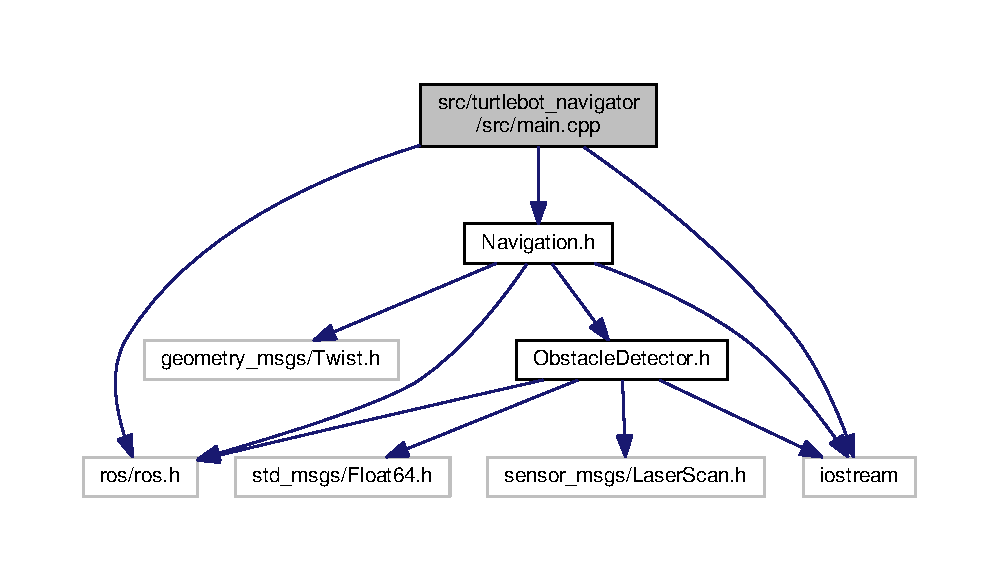
\includegraphics[width=350pt]{src_2main_8cpp__incl}
\end{center}
\end{figure}
\subsection*{Functions}
\begin{DoxyCompactItemize}
\item 
int \hyperlink{src_2main_8cpp_a3c04138a5bfe5d72780bb7e82a18e627}{main} (int argc, char $\ast$$\ast$argv)
\end{DoxyCompactItemize}


\subsection{Function Documentation}
\index{src/main.\+cpp@{src/main.\+cpp}!main@{main}}
\index{main@{main}!src/main.\+cpp@{src/main.\+cpp}}
\subsubsection[{\texorpdfstring{main(int argc, char $\ast$$\ast$argv)}{main(int argc, char **argv)}}]{\setlength{\rightskip}{0pt plus 5cm}int main (
\begin{DoxyParamCaption}
\item[{int}]{argc, }
\item[{char $\ast$$\ast$}]{argv}
\end{DoxyParamCaption}
)}\hypertarget{src_2main_8cpp_a3c04138a5bfe5d72780bb7e82a18e627}{}\label{src_2main_8cpp_a3c04138a5bfe5d72780bb7e82a18e627}

\hypertarget{test_2main_8cpp}{}\section{src/turtlebot\+\_\+navigator/test/main.cpp File Reference}
\label{test_2main_8cpp}\index{src/turtlebot\+\_\+navigator/test/main.\+cpp@{src/turtlebot\+\_\+navigator/test/main.\+cpp}}
{\ttfamily \#include $<$ros/ros.\+h$>$}\\*
{\ttfamily \#include $<$gtest/gtest.\+h$>$}\\*
Include dependency graph for main.\+cpp\+:
\nopagebreak
\begin{figure}[H]
\begin{center}
\leavevmode
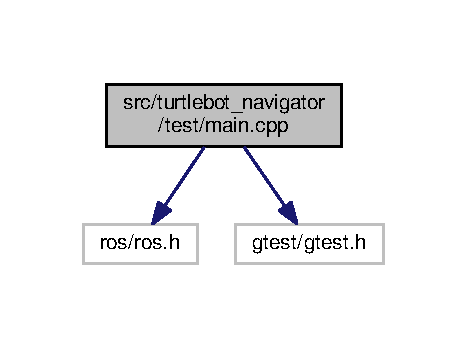
\includegraphics[width=224pt]{test_2main_8cpp__incl}
\end{center}
\end{figure}
\subsection*{Functions}
\begin{DoxyCompactItemize}
\item 
int \hyperlink{test_2main_8cpp_a3c04138a5bfe5d72780bb7e82a18e627}{main} (int argc, char $\ast$$\ast$argv)
\end{DoxyCompactItemize}


\subsection{Function Documentation}
\index{test/main.\+cpp@{test/main.\+cpp}!main@{main}}
\index{main@{main}!test/main.\+cpp@{test/main.\+cpp}}
\subsubsection[{\texorpdfstring{main(int argc, char $\ast$$\ast$argv)}{main(int argc, char **argv)}}]{\setlength{\rightskip}{0pt plus 5cm}int main (
\begin{DoxyParamCaption}
\item[{int}]{argc, }
\item[{char $\ast$$\ast$}]{argv}
\end{DoxyParamCaption}
)}\hypertarget{test_2main_8cpp_a3c04138a5bfe5d72780bb7e82a18e627}{}\label{test_2main_8cpp_a3c04138a5bfe5d72780bb7e82a18e627}

\hypertarget{_navigation_8cpp}{}\section{src/turtlebot\+\_\+navigator/src/\+Navigation.cpp File Reference}
\label{_navigation_8cpp}\index{src/turtlebot\+\_\+navigator/src/\+Navigation.\+cpp@{src/turtlebot\+\_\+navigator/src/\+Navigation.\+cpp}}


Describes the \hyperlink{class_navigation}{Navigation} class.  


{\ttfamily \#include $<$ros/ros.\+h$>$}\\*
{\ttfamily \#include $<$Navigation.\+h$>$}\\*
{\ttfamily \#include $<$Obstacle\+Detector.\+h$>$}\\*
{\ttfamily \#include $<$geometry\+\_\+msgs/\+Twist.\+h$>$}\\*
{\ttfamily \#include $<$iostream$>$}\\*
Include dependency graph for Navigation.\+cpp\+:
\nopagebreak
\begin{figure}[H]
\begin{center}
\leavevmode
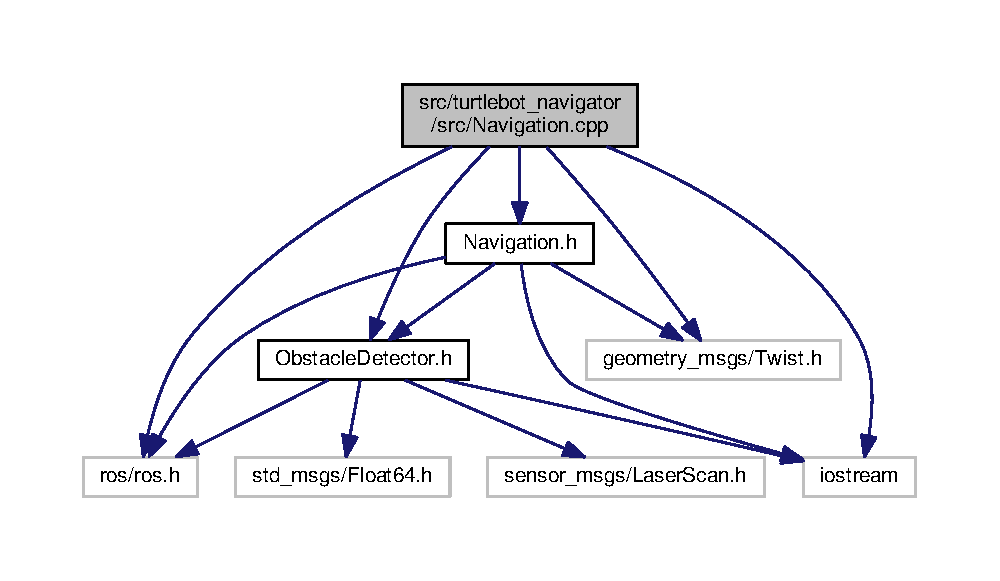
\includegraphics[width=350pt]{_navigation_8cpp__incl}
\end{center}
\end{figure}


\subsection{Detailed Description}
Describes the \hyperlink{class_navigation}{Navigation} class. 

M\+IT License

Copyright (c) 2019 Arpit Aggarwal Shantam Bajpai

Permission is hereby granted, free of charge, to any person obtaining a copy of this software and associated documentation files (the \char`\"{}\+Software\char`\"{}), to deal in the Software without restriction, including without limitation the rights to use, copy, modify, merge, publish, distribute, sublicense, and/or sell copies of the Software, and to permit persons to whom the Software is furnished to do so, subject to the following conditions\+:

The above copyright notice and this permission notice shall be included in all copies or substantial portions of the Software.

T\+HE S\+O\+F\+T\+W\+A\+RE IS P\+R\+O\+V\+I\+D\+ED \char`\"{}\+A\+S I\+S\char`\"{}, W\+I\+T\+H\+O\+UT W\+A\+R\+R\+A\+N\+TY OF A\+NY K\+I\+ND, E\+X\+P\+R\+E\+SS OR I\+M\+P\+L\+I\+ED, I\+N\+C\+L\+U\+D\+I\+NG B\+UT N\+OT L\+I\+M\+I\+T\+ED TO T\+HE W\+A\+R\+R\+A\+N\+T\+I\+ES OF M\+E\+R\+C\+H\+A\+N\+T\+A\+B\+I\+L\+I\+TY, F\+I\+T\+N\+E\+SS F\+OR A P\+A\+R\+T\+I\+C\+U\+L\+AR P\+U\+R\+P\+O\+SE A\+ND N\+O\+N\+I\+N\+F\+R\+I\+N\+G\+E\+M\+E\+NT. IN NO E\+V\+E\+NT S\+H\+A\+LL T\+HE A\+U\+T\+H\+O\+RS OR C\+O\+P\+Y\+R\+I\+G\+HT H\+O\+L\+D\+E\+RS BE L\+I\+A\+B\+LE F\+OR A\+NY C\+L\+A\+IM, D\+A\+M\+A\+G\+ES OR O\+T\+H\+ER L\+I\+A\+B\+I\+L\+I\+TY, W\+H\+E\+T\+H\+ER IN AN A\+C\+T\+I\+ON OF C\+O\+N\+T\+R\+A\+CT, T\+O\+RT OR O\+T\+H\+E\+R\+W\+I\+SE, A\+R\+I\+S\+I\+NG F\+R\+OM, O\+UT OF OR IN C\+O\+N\+N\+E\+C\+T\+I\+ON W\+I\+TH T\+HE S\+O\+F\+T\+W\+A\+RE OR T\+HE U\+SE OR O\+T\+H\+ER D\+E\+A\+L\+I\+N\+GS IN T\+HE S\+O\+F\+T\+W\+A\+RE.

\begin{DoxyCopyright}{Copyright}
M\+IT License 
\end{DoxyCopyright}

\hypertarget{_obstacle_detector_8cpp}{}\section{src/turtlebot\+\_\+navigator/src/\+Obstacle\+Detector.cpp File Reference}
\label{_obstacle_detector_8cpp}\index{src/turtlebot\+\_\+navigator/src/\+Obstacle\+Detector.\+cpp@{src/turtlebot\+\_\+navigator/src/\+Obstacle\+Detector.\+cpp}}


Implements the methods of the \hyperlink{class_obstacle_detector}{Obstacle\+Detector} class.  


{\ttfamily \#include $<$ros/ros.\+h$>$}\\*
{\ttfamily \#include $<$Obstacle\+Detector.\+h$>$}\\*
{\ttfamily \#include $<$std\+\_\+msgs/\+Float64.\+h$>$}\\*
{\ttfamily \#include $<$sensor\+\_\+msgs/\+Laser\+Scan.\+h$>$}\\*
{\ttfamily \#include $<$iostream$>$}\\*
Include dependency graph for Obstacle\+Detector.\+cpp\+:
\nopagebreak
\begin{figure}[H]
\begin{center}
\leavevmode
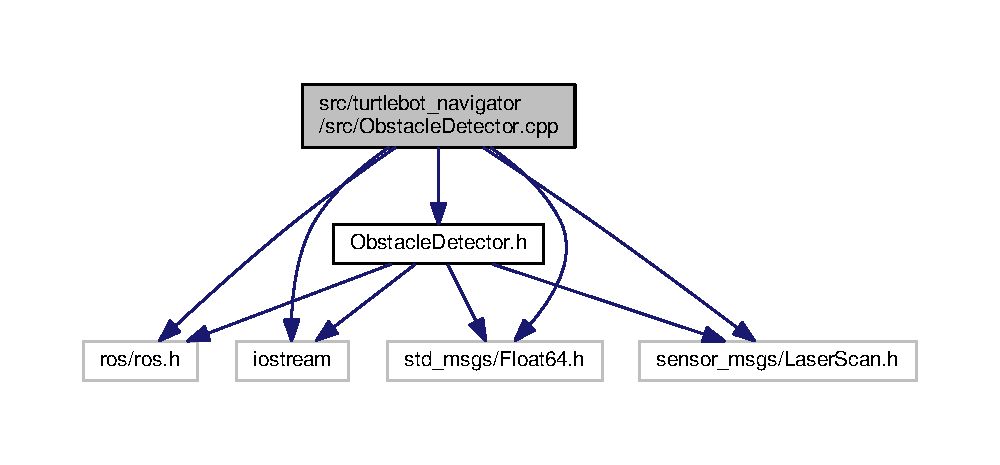
\includegraphics[width=350pt]{_obstacle_detector_8cpp__incl}
\end{center}
\end{figure}


\subsection{Detailed Description}
Implements the methods of the \hyperlink{class_obstacle_detector}{Obstacle\+Detector} class. 

M\+IT License

Copyright (c) 2019 Arpit Aggarwal Shantam Bajpai

Permission is hereby granted, free of charge, to any person obtaining a copy of this software and associated documentation files (the \char`\"{}\+Software\char`\"{}), to deal in the Software without restriction, including without limitation the rights to use, copy, modify, merge, publish, distribute, sublicense, and/or sell copies of the Software, and to permit persons to whom the Software is furnished to do so, subject to the following conditions\+:

The above copyright notice and this permission notice shall be included in all copies or substantial portions of the Software.

T\+HE S\+O\+F\+T\+W\+A\+RE IS P\+R\+O\+V\+I\+D\+ED \char`\"{}\+A\+S I\+S\char`\"{}, W\+I\+T\+H\+O\+UT W\+A\+R\+R\+A\+N\+TY OF A\+NY K\+I\+ND, E\+X\+P\+R\+E\+SS OR I\+M\+P\+L\+I\+ED, I\+N\+C\+L\+U\+D\+I\+NG B\+UT N\+OT L\+I\+M\+I\+T\+ED TO T\+HE W\+A\+R\+R\+A\+N\+T\+I\+ES OF M\+E\+R\+C\+H\+A\+N\+T\+A\+B\+I\+L\+I\+TY, F\+I\+T\+N\+E\+SS F\+OR A P\+A\+R\+T\+I\+C\+U\+L\+AR P\+U\+R\+P\+O\+SE A\+ND N\+O\+N\+I\+N\+F\+R\+I\+N\+G\+E\+M\+E\+NT. IN NO E\+V\+E\+NT S\+H\+A\+LL T\+HE A\+U\+T\+H\+O\+RS OR C\+O\+P\+Y\+R\+I\+G\+HT H\+O\+L\+D\+E\+RS BE L\+I\+A\+B\+LE F\+OR A\+NY C\+L\+A\+IM, D\+A\+M\+A\+G\+ES OR O\+T\+H\+ER L\+I\+A\+B\+I\+L\+I\+TY, W\+H\+E\+T\+H\+ER IN AN A\+C\+T\+I\+ON OF C\+O\+N\+T\+R\+A\+CT, T\+O\+RT OR O\+T\+H\+E\+R\+W\+I\+SE, A\+R\+I\+S\+I\+NG F\+R\+OM, O\+UT OF OR IN C\+O\+N\+N\+E\+C\+T\+I\+ON W\+I\+TH T\+HE S\+O\+F\+T\+W\+A\+RE OR T\+HE U\+SE OR O\+T\+H\+ER D\+E\+A\+L\+I\+N\+GS IN T\+HE S\+O\+F\+T\+W\+A\+RE.

\begin{DoxyCopyright}{Copyright}
M\+IT License 
\end{DoxyCopyright}

\hypertarget{_navigation_test_8cpp}{}\section{src/turtlebot\+\_\+navigator/test/\+Navigation\+Test.cpp File Reference}
\label{_navigation_test_8cpp}\index{src/turtlebot\+\_\+navigator/test/\+Navigation\+Test.\+cpp@{src/turtlebot\+\_\+navigator/test/\+Navigation\+Test.\+cpp}}


Test cases for \hyperlink{_navigation_test_8cpp}{Navigation\+Test.\+cpp} file.  


{\ttfamily \#include $<$gtest/gtest.\+h$>$}\\*
{\ttfamily \#include $<$ros/ros.\+h$>$}\\*
{\ttfamily \#include $<$Navigation.\+h$>$}\\*
{\ttfamily \#include $<$iostream$>$}\\*
Include dependency graph for Navigation\+Test.\+cpp\+:
\nopagebreak
\begin{figure}[H]
\begin{center}
\leavevmode
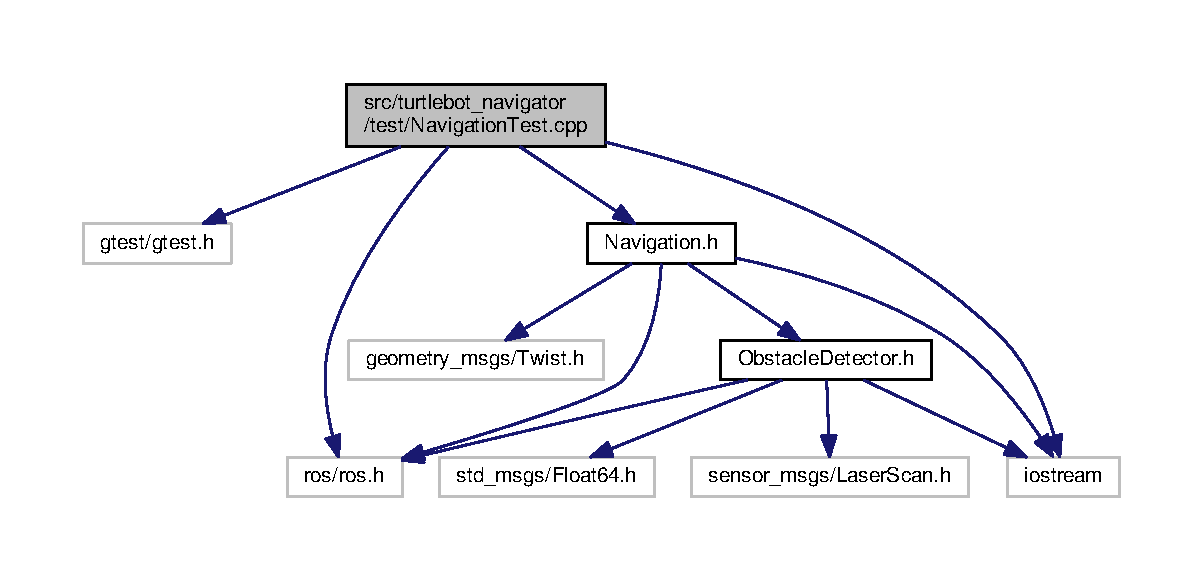
\includegraphics[width=350pt]{_navigation_test_8cpp__incl}
\end{center}
\end{figure}
\subsection*{Functions}
\begin{DoxyCompactItemize}
\item 
\hyperlink{_navigation_test_8cpp_af2f528f4cd2f685bd319ca4aa7eab1f5}{T\+E\+ST} (Navigation\+Test, Navigation\+Test)
\begin{DoxyCompactList}\small\item\em Tests the object creation of the class \hyperlink{class_navigation}{Navigation}. \end{DoxyCompactList}\item 
\hyperlink{_navigation_test_8cpp_a155a43a2e8f70fdac2175b3b29c76a13}{T\+E\+ST} (Navigation\+Test, move\+Method\+Test)
\end{DoxyCompactItemize}


\subsection{Detailed Description}
Test cases for \hyperlink{_navigation_test_8cpp}{Navigation\+Test.\+cpp} file. 

M\+IT License

Copyright (c) 2019 Arpit Aggarwal Shantam Bajpai

Permission is hereby granted, free of charge, to any person obtaining a copy of this software and associated documentation files (the \char`\"{}\+Software\char`\"{}), to deal in the Software without restriction, including without limitation the rights to use, copy, modify, merge, publish, distribute, sublicense, and/or sell copies of the Software, and to permit persons to whom the Software is furnished to do so, subject to the following conditions\+:

The above copyright notice and this permission notice shall be included in all copies or substantial portions of the Software.

T\+HE S\+O\+F\+T\+W\+A\+RE IS P\+R\+O\+V\+I\+D\+ED \char`\"{}\+A\+S I\+S\char`\"{}, W\+I\+T\+H\+O\+UT W\+A\+R\+R\+A\+N\+TY OF A\+NY K\+I\+ND, E\+X\+P\+R\+E\+SS OR I\+M\+P\+L\+I\+ED, I\+N\+C\+L\+U\+D\+I\+NG B\+UT N\+OT L\+I\+M\+I\+T\+ED TO T\+HE W\+A\+R\+R\+A\+N\+T\+I\+ES OF M\+E\+R\+C\+H\+A\+N\+T\+A\+B\+I\+L\+I\+TY, F\+I\+T\+N\+E\+SS F\+OR A P\+A\+R\+T\+I\+C\+U\+L\+AR P\+U\+R\+P\+O\+SE A\+ND N\+O\+N\+I\+N\+F\+R\+I\+N\+G\+E\+M\+E\+NT. IN NO E\+V\+E\+NT S\+H\+A\+LL T\+HE A\+U\+T\+H\+O\+RS OR C\+O\+P\+Y\+R\+I\+G\+HT H\+O\+L\+D\+E\+RS BE L\+I\+A\+B\+LE F\+OR A\+NY C\+L\+A\+IM, D\+A\+M\+A\+G\+ES OR O\+T\+H\+ER L\+I\+A\+B\+I\+L\+I\+TY, W\+H\+E\+T\+H\+ER IN AN A\+C\+T\+I\+ON OF C\+O\+N\+T\+R\+A\+CT, T\+O\+RT OR O\+T\+H\+E\+R\+W\+I\+SE, A\+R\+I\+S\+I\+NG F\+R\+OM, O\+UT OF OR IN C\+O\+N\+N\+E\+C\+T\+I\+ON W\+I\+TH T\+HE S\+O\+F\+T\+W\+A\+RE OR T\+HE U\+SE OR O\+T\+H\+ER D\+E\+A\+L\+I\+N\+GS IN T\+HE S\+O\+F\+T\+W\+A\+RE.

\begin{DoxyCopyright}{Copyright}
M\+IT License 
\end{DoxyCopyright}


\subsection{Function Documentation}
\index{Navigation\+Test.\+cpp@{Navigation\+Test.\+cpp}!T\+E\+ST@{T\+E\+ST}}
\index{T\+E\+ST@{T\+E\+ST}!Navigation\+Test.\+cpp@{Navigation\+Test.\+cpp}}
\subsubsection[{\texorpdfstring{T\+E\+S\+T(\+Navigation\+Test, Navigation\+Test)}{TEST(NavigationTest, NavigationTest)}}]{\setlength{\rightskip}{0pt plus 5cm}T\+E\+ST (
\begin{DoxyParamCaption}
\item[{Navigation\+Test}]{, }
\item[{Navigation\+Test}]{}
\end{DoxyParamCaption}
)}\hypertarget{_navigation_test_8cpp_af2f528f4cd2f685bd319ca4aa7eab1f5}{}\label{_navigation_test_8cpp_af2f528f4cd2f685bd319ca4aa7eab1f5}


Tests the object creation of the class \hyperlink{class_navigation}{Navigation}. 


\begin{DoxyParams}{Parameters}
{\em Navigation\+Test} & gtest framework \\
\hline
{\em Navigation\+Test} & Name of the test \\
\hline
\end{DoxyParams}
\begin{DoxyReturn}{Returns}
none 
\end{DoxyReturn}
\index{Navigation\+Test.\+cpp@{Navigation\+Test.\+cpp}!T\+E\+ST@{T\+E\+ST}}
\index{T\+E\+ST@{T\+E\+ST}!Navigation\+Test.\+cpp@{Navigation\+Test.\+cpp}}
\subsubsection[{\texorpdfstring{T\+E\+S\+T(\+Navigation\+Test, move\+Method\+Test)}{TEST(NavigationTest, moveMethodTest)}}]{\setlength{\rightskip}{0pt plus 5cm}T\+E\+ST (
\begin{DoxyParamCaption}
\item[{Navigation\+Test}]{, }
\item[{move\+Method\+Test}]{}
\end{DoxyParamCaption}
)}\hypertarget{_navigation_test_8cpp_a155a43a2e8f70fdac2175b3b29c76a13}{}\label{_navigation_test_8cpp_a155a43a2e8f70fdac2175b3b29c76a13}

\hypertarget{_obstacle_detector_test_8cpp}{}\section{src/turtlebot\+\_\+navigator/test/\+Obstacle\+Detector\+Test.cpp File Reference}
\label{_obstacle_detector_test_8cpp}\index{src/turtlebot\+\_\+navigator/test/\+Obstacle\+Detector\+Test.\+cpp@{src/turtlebot\+\_\+navigator/test/\+Obstacle\+Detector\+Test.\+cpp}}


Test cases for \hyperlink{_obstacle_detector_8cpp}{Obstacle\+Detector.\+cpp} file.  


{\ttfamily \#include $<$ros/ros.\+h$>$}\\*
{\ttfamily \#include $<$gtest/gtest.\+h$>$}\\*
{\ttfamily \#include $<$std\+\_\+msgs/\+Float64.\+h$>$}\\*
{\ttfamily \#include $<$sensor\+\_\+msgs/\+Laser\+Scan.\+h$>$}\\*
{\ttfamily \#include $<$Obstacle\+Detector.\+h$>$}\\*
{\ttfamily \#include $<$iostream$>$}\\*
Include dependency graph for Obstacle\+Detector\+Test.\+cpp\+:
\nopagebreak
\begin{figure}[H]
\begin{center}
\leavevmode
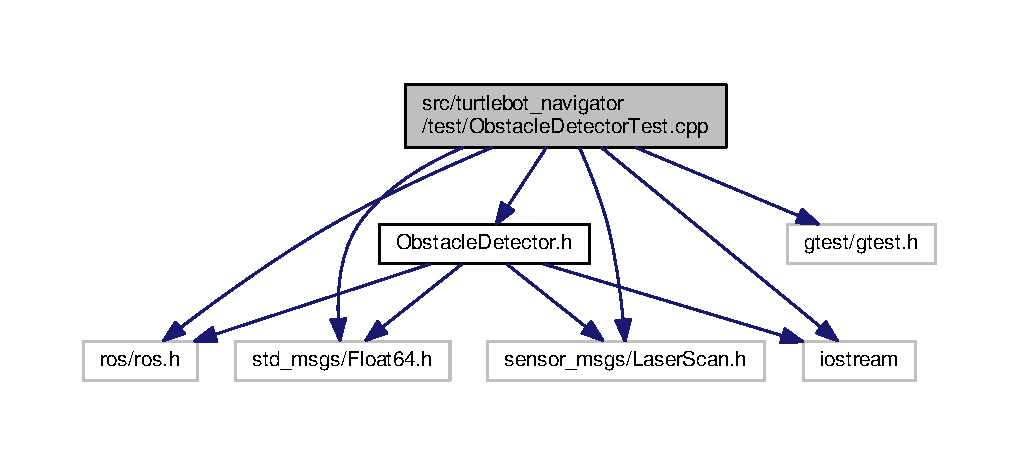
\includegraphics[width=350pt]{_obstacle_detector_test_8cpp__incl}
\end{center}
\end{figure}
\subsection*{Functions}
\begin{DoxyCompactItemize}
\item 
\hyperlink{_obstacle_detector_test_8cpp_ae91b9562af8e7251b2a46768ccb62d63}{T\+E\+ST} (Obstacle\+Detector\+Test, Obstacle\+Detector\+Test)
\begin{DoxyCompactList}\small\item\em Tests the object creation of the class \hyperlink{class_obstacle_detector}{Obstacle\+Detector}. \end{DoxyCompactList}\item 
\hyperlink{_obstacle_detector_test_8cpp_a0d4e42fe58ccc5feff9aa2d6d6e553fa}{T\+E\+ST} (Obstacle\+Detector\+Test, Collision\+Method\+Test)
\begin{DoxyCompactList}\small\item\em Tests the get\+Is\+Collision method of the class \hyperlink{class_obstacle_detector}{Obstacle\+Detector}. \end{DoxyCompactList}\item 
\hyperlink{_obstacle_detector_test_8cpp_a663fd288b0c65ac9c868e864ccc37bac}{T\+E\+ST} (Obstacle\+Detector\+Test, Laser\+Callback\+Method\+Test)
\begin{DoxyCompactList}\small\item\em Tests the laser\+Callback method of the class \hyperlink{class_obstacle_detector}{Obstacle\+Detector}. \end{DoxyCompactList}\item 
\hyperlink{_obstacle_detector_test_8cpp_a643f3ed26df4e2ceb035f206a9b7242b}{T\+E\+ST} (Obstacle\+Detector\+Test, Dist\+Callback\+Method\+Test)
\begin{DoxyCompactList}\small\item\em Tests the dist\+Callback method of the class \hyperlink{class_obstacle_detector}{Obstacle\+Detector}. \end{DoxyCompactList}\end{DoxyCompactItemize}


\subsection{Detailed Description}
Test cases for \hyperlink{_obstacle_detector_8cpp}{Obstacle\+Detector.\+cpp} file. 

M\+IT License

Copyright (c) 2019 Arpit Aggarwal Shantam Bajpai

Permission is hereby granted, free of charge, to any person obtaining a copy of this software and associated documentation files (the \char`\"{}\+Software\char`\"{}), to deal in the Software without restriction, including without limitation the rights to use, copy, modify, merge, publish, distribute, sublicense, and/or sell copies of the Software, and to permit persons to whom the Software is furnished to do so, subject to the following conditions\+:

The above copyright notice and this permission notice shall be included in all copies or substantial portions of the Software.

T\+HE S\+O\+F\+T\+W\+A\+RE IS P\+R\+O\+V\+I\+D\+ED \char`\"{}\+A\+S I\+S\char`\"{}, W\+I\+T\+H\+O\+UT W\+A\+R\+R\+A\+N\+TY OF A\+NY K\+I\+ND, E\+X\+P\+R\+E\+SS OR I\+M\+P\+L\+I\+ED, I\+N\+C\+L\+U\+D\+I\+NG B\+UT N\+OT L\+I\+M\+I\+T\+ED TO T\+HE W\+A\+R\+R\+A\+N\+T\+I\+ES OF M\+E\+R\+C\+H\+A\+N\+T\+A\+B\+I\+L\+I\+TY, F\+I\+T\+N\+E\+SS F\+OR A P\+A\+R\+T\+I\+C\+U\+L\+AR P\+U\+R\+P\+O\+SE A\+ND N\+O\+N\+I\+N\+F\+R\+I\+N\+G\+E\+M\+E\+NT. IN NO E\+V\+E\+NT S\+H\+A\+LL T\+HE A\+U\+T\+H\+O\+RS OR C\+O\+P\+Y\+R\+I\+G\+HT H\+O\+L\+D\+E\+RS BE L\+I\+A\+B\+LE F\+OR A\+NY C\+L\+A\+IM, D\+A\+M\+A\+G\+ES OR O\+T\+H\+ER L\+I\+A\+B\+I\+L\+I\+TY, W\+H\+E\+T\+H\+ER IN AN A\+C\+T\+I\+ON OF C\+O\+N\+T\+R\+A\+CT, T\+O\+RT OR O\+T\+H\+E\+R\+W\+I\+SE, A\+R\+I\+S\+I\+NG F\+R\+OM, O\+UT OF OR IN C\+O\+N\+N\+E\+C\+T\+I\+ON W\+I\+TH T\+HE S\+O\+F\+T\+W\+A\+RE OR T\+HE U\+SE OR O\+T\+H\+ER D\+E\+A\+L\+I\+N\+GS IN T\+HE S\+O\+F\+T\+W\+A\+RE.

\begin{DoxyCopyright}{Copyright}
M\+IT License 
\end{DoxyCopyright}


\subsection{Function Documentation}
\index{Obstacle\+Detector\+Test.\+cpp@{Obstacle\+Detector\+Test.\+cpp}!T\+E\+ST@{T\+E\+ST}}
\index{T\+E\+ST@{T\+E\+ST}!Obstacle\+Detector\+Test.\+cpp@{Obstacle\+Detector\+Test.\+cpp}}
\subsubsection[{\texorpdfstring{T\+E\+S\+T(\+Obstacle\+Detector\+Test, Obstacle\+Detector\+Test)}{TEST(ObstacleDetectorTest, ObstacleDetectorTest)}}]{\setlength{\rightskip}{0pt plus 5cm}T\+E\+ST (
\begin{DoxyParamCaption}
\item[{Obstacle\+Detector\+Test}]{, }
\item[{Obstacle\+Detector\+Test}]{}
\end{DoxyParamCaption}
)}\hypertarget{_obstacle_detector_test_8cpp_ae91b9562af8e7251b2a46768ccb62d63}{}\label{_obstacle_detector_test_8cpp_ae91b9562af8e7251b2a46768ccb62d63}


Tests the object creation of the class \hyperlink{class_obstacle_detector}{Obstacle\+Detector}. 


\begin{DoxyParams}{Parameters}
{\em Obstacle\+Detector\+Test} & gtest framework \\
\hline
{\em Obstacle\+Detector\+Test} & Name of the test \\
\hline
\end{DoxyParams}
\begin{DoxyReturn}{Returns}
none 
\end{DoxyReturn}
\index{Obstacle\+Detector\+Test.\+cpp@{Obstacle\+Detector\+Test.\+cpp}!T\+E\+ST@{T\+E\+ST}}
\index{T\+E\+ST@{T\+E\+ST}!Obstacle\+Detector\+Test.\+cpp@{Obstacle\+Detector\+Test.\+cpp}}
\subsubsection[{\texorpdfstring{T\+E\+S\+T(\+Obstacle\+Detector\+Test, Collision\+Method\+Test)}{TEST(ObstacleDetectorTest, CollisionMethodTest)}}]{\setlength{\rightskip}{0pt plus 5cm}T\+E\+ST (
\begin{DoxyParamCaption}
\item[{Obstacle\+Detector\+Test}]{, }
\item[{Collision\+Method\+Test}]{}
\end{DoxyParamCaption}
)}\hypertarget{_obstacle_detector_test_8cpp_a0d4e42fe58ccc5feff9aa2d6d6e553fa}{}\label{_obstacle_detector_test_8cpp_a0d4e42fe58ccc5feff9aa2d6d6e553fa}


Tests the get\+Is\+Collision method of the class \hyperlink{class_obstacle_detector}{Obstacle\+Detector}. 


\begin{DoxyParams}{Parameters}
{\em Obstacle\+Detector\+Test} & gtest framework \\
\hline
{\em Collision\+Method\+Test} & Name of the test \\
\hline
\end{DoxyParams}
\begin{DoxyReturn}{Returns}
none 
\end{DoxyReturn}
\index{Obstacle\+Detector\+Test.\+cpp@{Obstacle\+Detector\+Test.\+cpp}!T\+E\+ST@{T\+E\+ST}}
\index{T\+E\+ST@{T\+E\+ST}!Obstacle\+Detector\+Test.\+cpp@{Obstacle\+Detector\+Test.\+cpp}}
\subsubsection[{\texorpdfstring{T\+E\+S\+T(\+Obstacle\+Detector\+Test, Laser\+Callback\+Method\+Test)}{TEST(ObstacleDetectorTest, LaserCallbackMethodTest)}}]{\setlength{\rightskip}{0pt plus 5cm}T\+E\+ST (
\begin{DoxyParamCaption}
\item[{Obstacle\+Detector\+Test}]{, }
\item[{Laser\+Callback\+Method\+Test}]{}
\end{DoxyParamCaption}
)}\hypertarget{_obstacle_detector_test_8cpp_a663fd288b0c65ac9c868e864ccc37bac}{}\label{_obstacle_detector_test_8cpp_a663fd288b0c65ac9c868e864ccc37bac}


Tests the laser\+Callback method of the class \hyperlink{class_obstacle_detector}{Obstacle\+Detector}. 


\begin{DoxyParams}{Parameters}
{\em Obstacle\+Detector\+Test} & gtest framework \\
\hline
{\em Laser\+Callback\+Method\+Test} & Name of the test \\
\hline
\end{DoxyParams}
\begin{DoxyReturn}{Returns}
none 
\end{DoxyReturn}
\index{Obstacle\+Detector\+Test.\+cpp@{Obstacle\+Detector\+Test.\+cpp}!T\+E\+ST@{T\+E\+ST}}
\index{T\+E\+ST@{T\+E\+ST}!Obstacle\+Detector\+Test.\+cpp@{Obstacle\+Detector\+Test.\+cpp}}
\subsubsection[{\texorpdfstring{T\+E\+S\+T(\+Obstacle\+Detector\+Test, Dist\+Callback\+Method\+Test)}{TEST(ObstacleDetectorTest, DistCallbackMethodTest)}}]{\setlength{\rightskip}{0pt plus 5cm}T\+E\+ST (
\begin{DoxyParamCaption}
\item[{Obstacle\+Detector\+Test}]{, }
\item[{Dist\+Callback\+Method\+Test}]{}
\end{DoxyParamCaption}
)}\hypertarget{_obstacle_detector_test_8cpp_a643f3ed26df4e2ceb035f206a9b7242b}{}\label{_obstacle_detector_test_8cpp_a643f3ed26df4e2ceb035f206a9b7242b}


Tests the dist\+Callback method of the class \hyperlink{class_obstacle_detector}{Obstacle\+Detector}. 


\begin{DoxyParams}{Parameters}
{\em Obstacle\+Detector\+Test} & gtest framework \\
\hline
{\em Dist\+Callback\+Method\+Test} & Name of the test \\
\hline
\end{DoxyParams}
\begin{DoxyReturn}{Returns}
none 
\end{DoxyReturn}

%--- End generated contents ---

% Index
\backmatter
\newpage
\phantomsection
\clearemptydoublepage
\addcontentsline{toc}{chapter}{Index}
\printindex

\end{document}
